\section{Magnolia Shell}
As long as the architecture splits the functionality units into apps it is
logical to assume that there must be an environment that would host and
manipulate those apps. In Magnolia 5.0 such an environment is called
\texttt{MagnoliaShell}.

Magnolia Shell is the main part of Magnolia 5.0 user interface foundation.
Primarily the component is responsible for displaying and laying-out the apps
and for performing transitions between them, which makes it a core UI container
of the project.
MagnoliaShell is also highly important part of the architecture due to its
integration with other parts of the system.
 

\begin{figure}[H] \centering 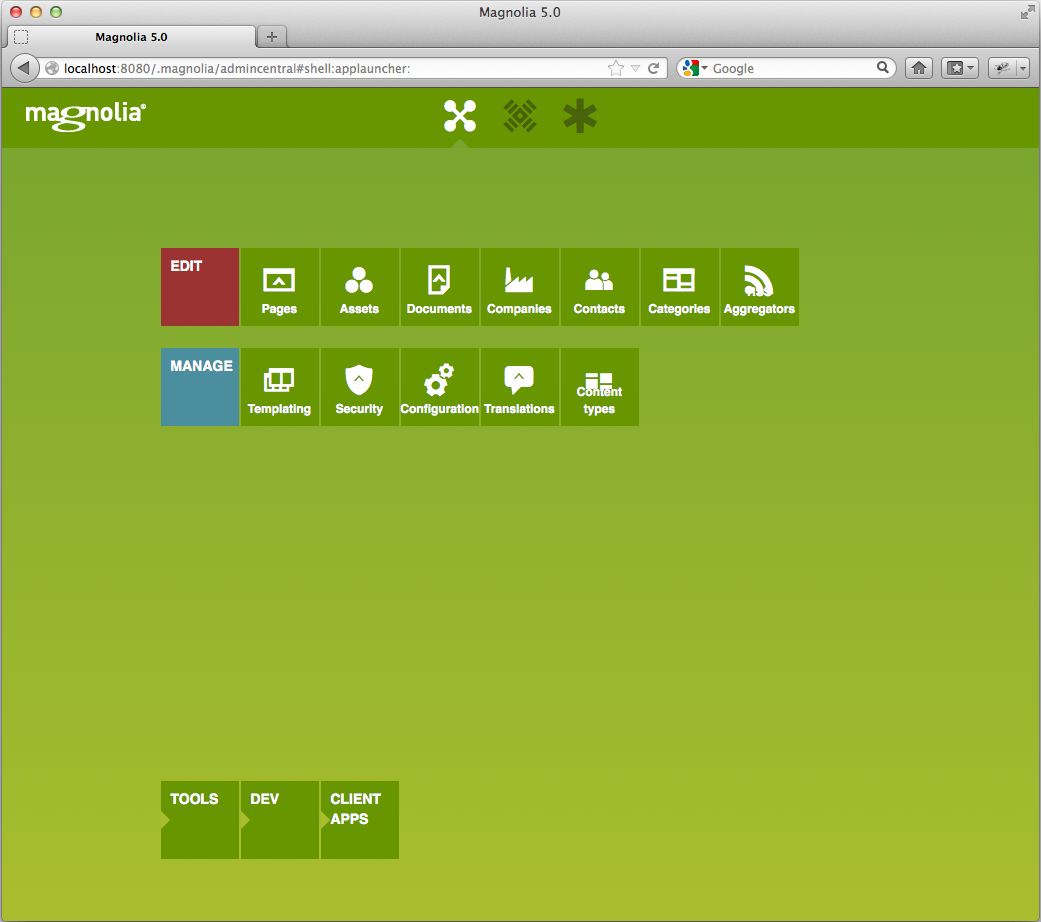
\includegraphics[width=\textwidth]{magnolia_shell.png}
	\caption{Magnolia Shell}
	\label{fig:m_shell}
\end{figure}

From the user interface point of view MagnoliaShell conceptually resembles the
browser viewport \cite{mshell_wiki}.
Actually, it contains two viewports (\texttt{ ShellViewport}): one for the apps
and one - for the shell apps.
 The \emph{ application framework } utilizes the viewports as containers in
 \texttt{AppController} and \texttt{ShellAppController} implementation.

\emph{Locations framework} is also connected with MagnoliaShell. The latter acts
as a buffer between client and server sides in fragment handling process. The
client-side implementation of MagnoliaShell subscribes to GWT's History API
events, based on a fragment it resolves which type of an app it has to launch
and instructs the server accordingly. On the server-side the
\texttt{LocationHistoryHandler} de-serializes the received fragment into a
\texttt{Location} instance which is handled by either \texttt{AppController} or
\texttt{ShellAppController}: based on the location parameters the correct
sub-app is launched. The other way around - an app is able to initiate a
navigation event (e.g. when switching between two app due to some server side
logic), at the end simply forcing the browser to update its fragment silently
(without sending an event to subscribers).
